\section{Mid-bunch slices and large-domain slices}
\label{app:slices}

\subsection{Mid-bunch slices: field and error side by side}
\label{app:slices-mid}

The distance sweeps of Section~\ref{sec:farfield} sample the far field. To
measure the mesh in the bunch core we slice through it and compare, pixel
by pixel, with an exact TSC-convolved reference: $64\times64$ planes, cell
$10^{-7}$\,m, $N=200$, $Q=-100$\,pC, $\gamma=10$ with momentum along $+y$.
Two cases share the positions and differ only in a $1.046$\,mrad rms
transverse divergence in $x$ (Figs.~\ref{fig:valforward} and
\ref{fig:valfluct}). A
separate unit-weight bunch (the first 200 of the 1000-particle seed-43 case
of Table~\ref{tab:configs}, $Q=-32$\,aC) propagates along $+y$ and is
different from the seed-42 mono-energetic bunch that moves along $+x$ in
the $\gamma=10$ case of Table~\ref{tab:slices}. It is binned on the
$32\times32\times16$ grid of cell $2\times10^{-7}$\,m and sliced at its
mid-plane (Fig.~\ref{fig:val1mrad}). In every panel of these $+y$ figures, $y$ is
horizontal and increases left to right, so the bunch moves rightwards and $y$
is the beam axis; the vertical axis is $x$ in the x-y cut and $z$ in the z-y
cut. The top row of each plate is a charge-density overview of the bunch, not
a field map; its three panels are the coordinate planes and its transverse
panels carry the ``beam axis (out of plane)'' note (see the caption of
Fig.~\ref{fig:valforward}). Each figure has
a field row with four columns ($E_x,E_y,E_z,E^2$); the forward and
$1$\,mrad figures carry an error row underneath, while the reference-only
fluctuation figure shows the electric and magnetic field rows alone. The three
components share one symmetric-logarithmic colour scale
and bar, and each component panel states its peak as a percentage of the
shared maximum. $E^2$ (or $B^2$) has its own logarithmic scale from $10^{-6}$
of the panel peak to the peak, with its own unit label. The error row is
logarithmic, floored at $10^{-6}$ and marked at the $10^{-3}$ gate. Pixels are
masked in light grey where the local field magnitude is below $10^{-3}$ of
the largest component peak on the plane. The forward case compares the mesh
plus fast shell against an order-4 adaptive Gauss--Legendre driver. The Lorentz-contracted
in-support quadrature of Section~\ref{sec:fastacc} is the present
reference; it differs from that driver at the few-percent level at the
closest node, so the in-support error pixels in these panels bound the
in-support error from above. The dark outline marks the TSC support.
The quantitative in-support statement is the fast-versus-arbiter $1.6\%$
at the worst node (Section~\ref{sec:fastacc}). The fluctuation panels show
the complete reference field; the binned momentum-spread case is carried
through the multi-velocity path (Appendix~\ref{app:multivel}).

\paragraph{Shell radius unit.}
The near-shell envelope measured in the crossover work, ``3 to 4 PIC
cells,'' assumed a mesh spacing $h=1/4$ of the PIC cell, so $R=3$ and
$R=4$ are 12 and 16 mesh nodes. On this grid the node spacing is $h=1$
PIC cell ($2\times10^{-7}$\,m), so the same $R=3/4$ is 3/4 mesh nodes, four
times smaller in physical units than the envelope configuration. At $R=3$
on an $h=1$ grid the shell covers 3 mesh nodes; the TSC support extends
$\pm1.5$ cells from each source, so the shell covers a fraction of the full
support. The measured plane errors at this radius are reported below.

\begin{figure}[t]
\centering
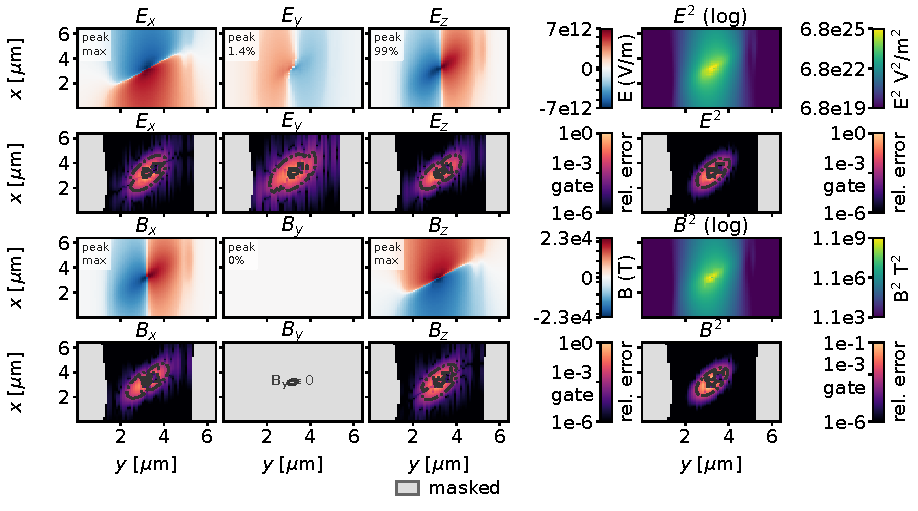
\includegraphics[width=\linewidth]{figs/val_forward_xy.pdf}
\caption{Forward-case validation ($N=200$, $Q=-100$\,pC,
$\gamma=10$ along $+y$, $64\times64$ planes, cell $10^{-7}$\,m; x-y plane
at $z=3.2\,\si{\micro\metre}$, with $y$ horizontal, the beam axis; the
z-y plane at $x=3.2\,\si{\micro\metre}$ is continued in
Fig.~\ref{fig:valforward}. \densityrow{} Below the density row, each image
carries the electric block first and the magnetic block second.
The electric block shows four columns $E_x,E_y,E_z,E^2$: the three components
share one symmetric-logarithmic scale and bar (the text gives the $E^2$ scale
and unit). Each component panel is labelled with its peak as a percentage of the
largest component peak on that plane (the shared colour scale): the panel that
sets the maximum reads \texttt{max}, peaks below one percent use one
significant figure (e.g.\ \texttt{.04\%}), and only an exactly zero peak reads
$0\%$; a small percentage means the component is faint on that scale. The
magnetic block shows the same layout for $B_x,B_y,B_z,B^2$. $B_y$ is
identically zero: its field panel is blank and its error panel is fully masked,
since the relative error of an identically zero component is undefined. Under
each field row lies a logarithmic error row, floored at $10^{-6}$ and marked at
the $10^{-3}$ gate, with light-grey pixels where the local field magnitude is
below $10^{-3}$ of the largest component peak on the plane; the dark outline
marks the TSC support. The in-support fast-versus-arbiter error against the
order-12 independent continuum reference is $1.6\%$ at the worst node. The
magnetic field is about $3.3\!\times\!10^{-9}$ of the $E$-dominated local
field at $\gamma=10$ (Section~\ref{sec:accuracy}).}
\label{fig:valforward}
\end{figure}

\begin{figure}[t]
\ContinuedFloat
\centering
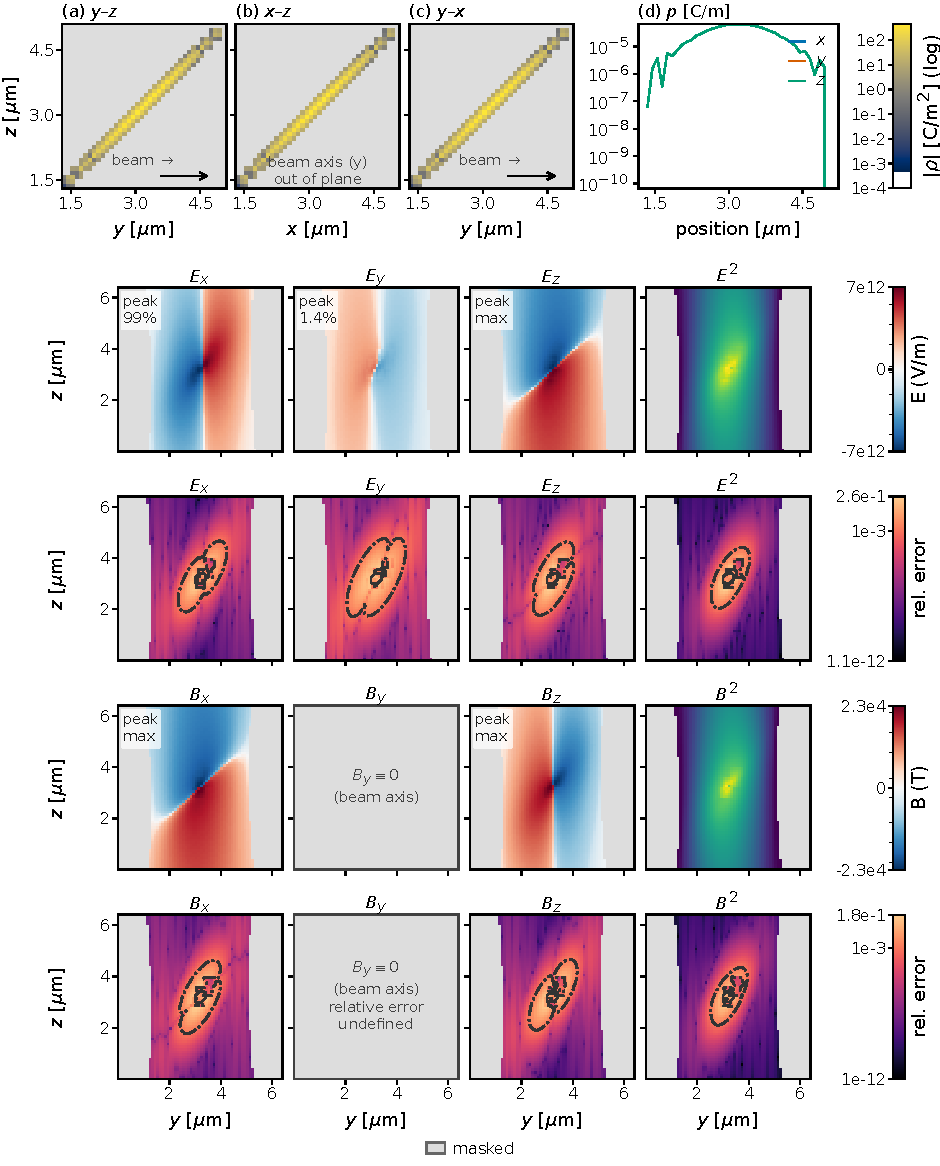
\includegraphics[width=\linewidth]{figs/val_forward_zy.pdf}
\caption{Forward-case validation (continued): z-y plane at
$x=3.2\,\si{\micro\metre}$, with the same electric/magnetic blocks,
colour scales, masks and error conventions as the x-y plane in
Fig.~\ref{fig:valforward}.}
\end{figure}

\begin{figure}[t]
\centering
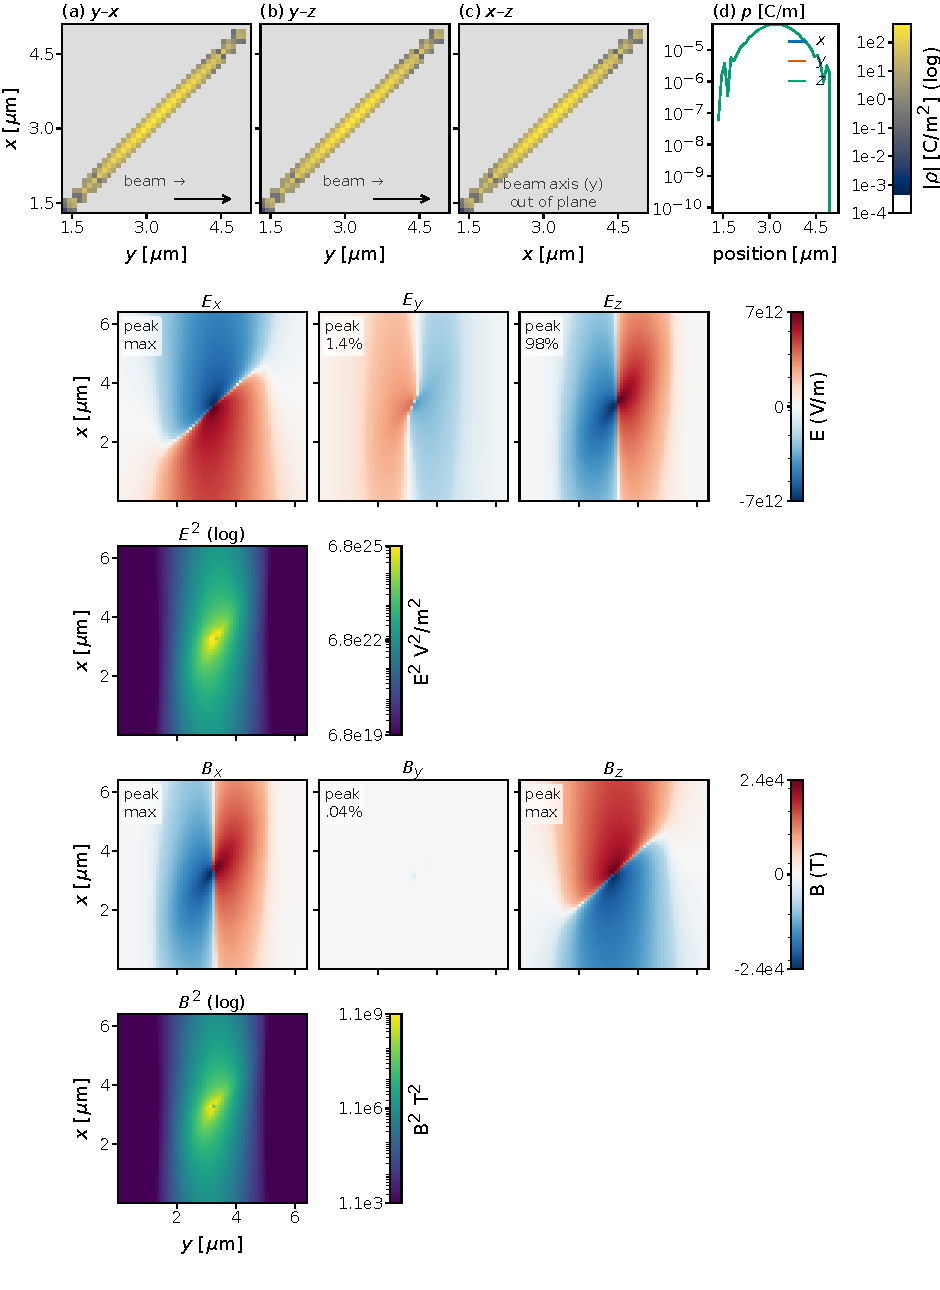
\includegraphics[width=\linewidth]{figs/val_fluct_xy.pdf}\\[2pt]
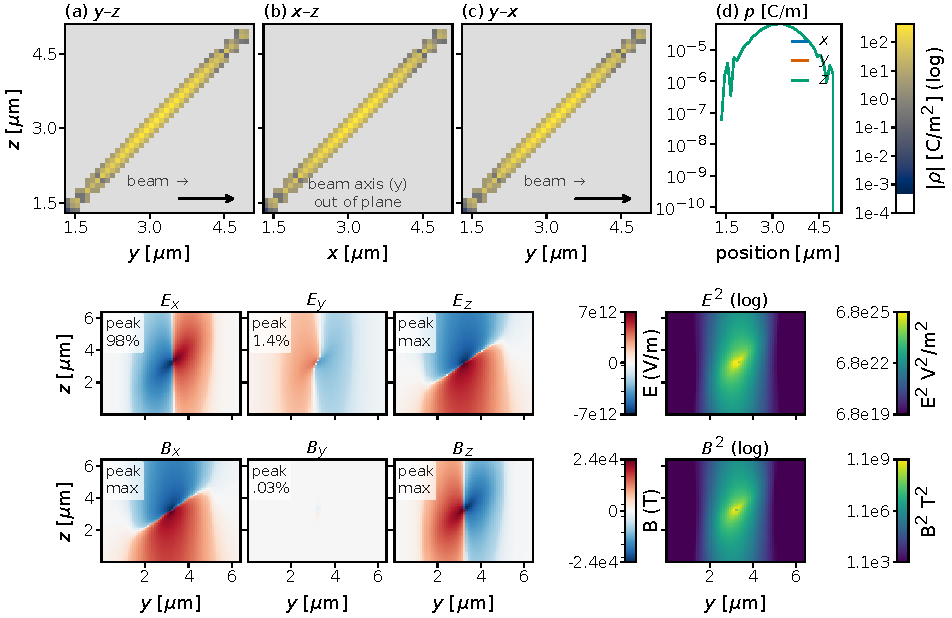
\includegraphics[width=\linewidth]{figs/val_fluct_zy.pdf}
\caption{Fluctuation-case reference with the same geometry and bunch as
Fig.~\ref{fig:valforward} but a $1.046$\,mrad rms $x$-divergence.
The top row repeats the charge-density overview of
Fig.~\ref{fig:valforward}. The upper and lower images are the x-y and z-y
planes, with $y$ horizontal and the beam axis; each carries the electric
field row first and the magnetic field row second, with the scales and masks
of Fig.~\ref{fig:valforward}. The panels show the order-12 independent
continuum reference; the $x$-divergence lifts $B_y$ off zero, although it
remains about $3\times10^{-4}$ of the dominant component. The corresponding
binned picBunch output is reported in Appendix~\ref{app:multivel}.}
\label{fig:valfluct}
\end{figure}

\begin{figure}[t]
\centering
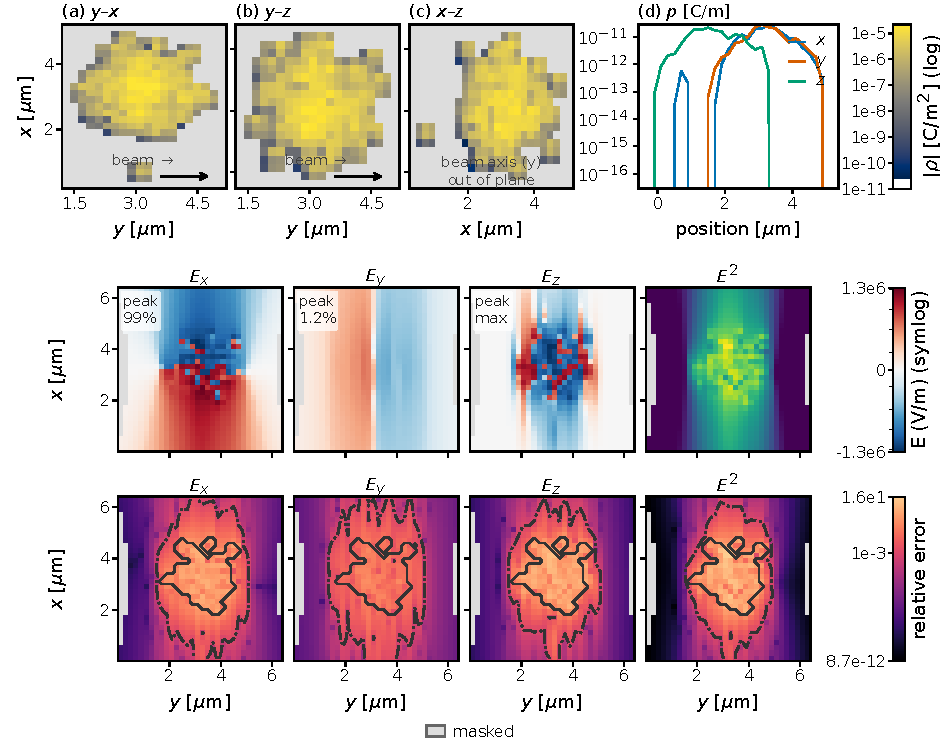
\includegraphics[width=\linewidth]{figs/val_1mrad_xy_E.pdf}\\[2pt]
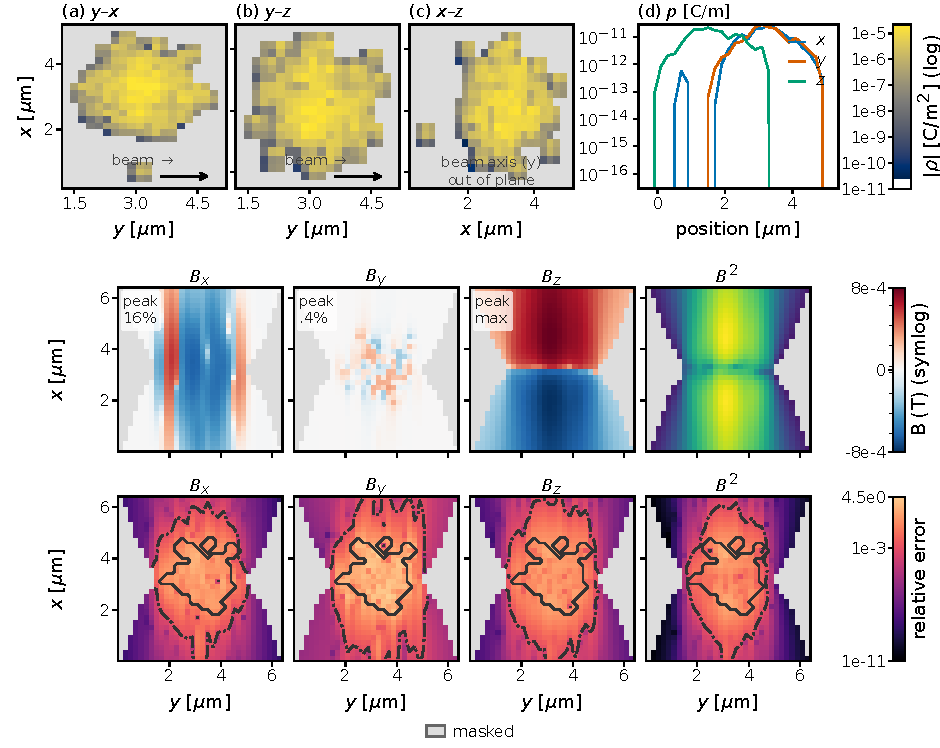
\includegraphics[width=\linewidth]{figs/val_1mrad_xy_B.pdf}
\caption{Binned $1$\,mrad case (seed-43 unit-weight bunch, $N=200$,
$Q=-32$\,aC, $\gamma=10$, $32\times32$ x-y plane at
$z=1.6\,\si{\micro\metre}$, cell $2\times10^{-7}$\,m), with the picBunch
velocity-binned field against the order-12 independent continuum reference.
The upper image is electric and the lower magnetic.}
\label{fig:val1mrad}
\end{figure}

\begin{table}[t]
\centering
\small
\caption{Mid-bunch slice statistics, mesh-only. Worst relative error per
component and fraction of unmasked plane pixels above $10^{-3}$ (unmasked
means the local field magnitude is at least $10^{-3}$ of the largest
component peak on the plane), x-y plane
at $z=1.60\,\si{\micro\metre}$ and z-y plane at $x=3.20\,\si{\micro\metre}$,
$N=1000$, $32\times32\times16$, cell $2\times10^{-7}$\,m, mesh against the
independent exact TSC driver (FP64 quadrature, order $4$, max level $5$,
tolerance $10^{-3}$). The $\gamma=10$ case is the seed-42 mono-energetic
bunch, which moves along $+x$ ($B_x\equiv0$);
$x$ is horizontal in the x-y cut and is the beam axis there, while $y$ is
horizontal in the z-y cut (beam out of plane) and $z$ vertical. Node spacing $h=1$ PIC cell; no near shell.
Measured on \texttt{rosi\_v100} (V100, v0.9.2; the near-shell numbers in
the text below this table are the JURECA H100 v0.9.2 runs, so this
mesh-only table and those near-shell values are on different hosts).
The $\gamma=1$ reference is stationary (no beam axis) and uses the archived
tolerance $10^{-4}$ (driver floor $9.075\times10^{-4}$, 14 not converged).}
\label{tab:slices}
\begin{tabular}{llrr}
\toprule
plane & component & worst rel. err & frac $>10^{-3}$ \\
\midrule
\multicolumn{4}{l}{\emph{$\gamma=10$ (beam axis $+x$; $B_x\equiv0$)}} \\
x-y ($z\!=\!1.60\,\si{\micro\metre}$) & $E_x$ & $1.81$ & $54.1\%$ \\
 & $E_y$ & $1.16\times10^{-1}$ & $49.9\%$ \\
 & $E_z$ & $5.33$ & $78.3\%$ \\
 & $B_y$ & $6.49\times10^{-1}$ & $72.7\%$ \\
 & $B_z$ & $3.77\times10^{-1}$ & $58.7\%$ \\
z-y ($x\!=\!3.20\,\si{\micro\metre}$) & $E_x$ & $5.06$ & $90.4\%$ \\
 & $E_y$ & $1.17\times10^{-1}$ & $61.1\%$ \\
 & $E_z$ & $1.92$ & $82.4\%$ \\
 & $B_y$ & $4.34\times10^{-1}$ & $80.9\%$ \\
 & $B_z$ & $7.16\times10^{-1}$ & $84.3\%$ \\
\midrule
\multicolumn{4}{l}{\emph{$\gamma=1$ (stationary; all $B\equiv0$)}} \\
x-y ($z\!=\!1.60\,\si{\micro\metre}$) & $E_x$ & $1.20\times10^{-1}$ & $22.8\%$ \\
 & $E_y$ & $1.34\times10^{-1}$ & $23.3\%$ \\
 & $E_z$ & $4.15\times10^{-1}$ & $74.7\%$ \\
z-y ($x\!=\!3.20\,\si{\micro\metre}$) & $E_x$ & $4.15\times10^{-1}$ & $49.6\%$ \\
 & $E_y$ & $1.37\times10^{-1}$ & $61.7\%$ \\
 & $E_z$ & $1.23\times10^{-1}$ & $53.9\%$ \\
\bottomrule
\end{tabular}
\end{table}

The error is largest where these planes cut the bunch core: the spectral
far-field convolution is not the dominant term there, and the maps show the
measured error concentrated at the beamed core and falling away toward the
plane edges. The far field is measured separately
(Table~\ref{tab:w4b}, Fig.~\ref{fig:Fw4b}); the near-shell contribution
is measured at the same geometry below.

\subsection{Near-shell accuracy and cost on the slice geometry}
\label{app:slices-runs}

On the same $N=1000$, $32\times32\times16$, cell $2\times10^{-7}$\,m
geometry (the seed-42 mono-energetic bunch of Table~\ref{tab:slices},
beam axis $+x$; not the seed-43 $+y$ bunch of
Fig.~\ref{fig:val1mrad}), the exact near shell was run at the radius the
envelope case
assumed, $R=3$ for $\gamma=1$ and $R=4$ for $\gamma=10$, in mesh nodes of
this $h=1$ grid; the mesh-only table and the near-shell numbers in this
subsection are the v0.9.2 library runs, in contrast to the v0.4.0
standalone driver of the crossover work. The mesh-only plane errors
(Table~\ref{tab:slices}) are $0.12$--$0.415$ for $\gamma=1$
($E_z$ in both planes) and $0.116$--$5.33$ for $\gamma=10$ (minimum $E_y$,
x-y; maximum $E_z$, x-y; beam axis $+x$, the $B_x$ component identically
zero): these planes cut the sources, the region
where the spectral convolution is not the dominant term. With the near
shell the worst per-component plane error is
$1.7\times10^{-3}$--$9.0\times10^{-3}$ for $\gamma=1$ (z-y plane $E_x$) and
$6.7\times10^{-2}$--$1.8\times10^{-1}$ for $\gamma=10$ (z-y plane $E_x$):
at $R=3/4$ on an $h=1$ grid the shell radius covers 3/4 mesh
nodes, which is a fraction of the TSC support extent, and the measured
residual is the mesh contribution outside the shell. The v0.4.0-driver
high ends, $0.1067$ for $\gamma=1$ and $0.5704$ for
$\gamma=10$, both sit on the same z-y $E_z$ plane's last domain row
($z=15$), where the v0.9.2 runs give $2.5\times10^{-5}$ and $0.0954$; the
driver edge values are artifacts, not a missing plane or
radius. The discrete
Gauss-law indicator, the Yee backward-difference $\mathrm{div}\,E$ residual
normalised to the peak deposited $\rho/\varepsilon_0$, moves from $0.3534$
to $0.0895$ for $\gamma=1$ and from $5.026$ to $0.399$ for $\gamma=10$,
against reference values $0.0904$ and $0.0814$: $\gamma=1$ reaches the
reference value, $\gamma=10$ drops $12.6\times$ and stays $4.9\times$
above it.

The assembly itself is not the limiting term: the tests of
Section~\ref{sec:nearsheet} show the tiled subtraction exact to roundoff,
so the residuals above are the mesh outside the shell. Runtime at
$N=1000$ is $4.3$ min for $\gamma=1$ and $32.7$ min for $\gamma=10$
(one 16-thread socket; the exact shell is the whole wall time); the
exact evaluator costs about $8\times$ more per pair at $\gamma=10$ than
at $\gamma=1$.

\subsection{Large-domain slices}
\label{app:slices-large}

Figure~\ref{fig:large} shows the $\gamma=10$ electric and magnetic field
and error on a $128\times128\times64$ domain, cell $2\times10^{-7}$\,m,
$N=100$, against the independent continuum at tolerance $10^{-3}$. The
electric block comes first and the magnetic block second in the same
figure, as in the per-$\gamma$ presentation. Fig.~\ref{fig:largeg1} is the
stationary-bunch case, with the electric block and the identically zero
magnetic field row. Figs.~\ref{fig:large}--\ref{fig:largeg1} use the
axial-$x$ geometry: the bunch moves along $+x$, so $B_x$, the field component
along the propagation axis, is identically zero. The x-y cut is longitudinal,
with the beam axis $x$ horizontal. The z-y cut is a transverse view of the
bunch: the beam axis $x$ is perpendicular to the page, so the horizontal
coordinate there is the transverse $y$, not the propagation direction, and
$z$ is vertical. This keeps the same horizontal $y$ and vertical $z$ as the
z-y cuts of the $+y$ figures, where the out-of-plane transverse axis is $x$. The
colour scale is set by the bunch, so the far decay is visible inside the
frame; the core error is the method error of the mesh where the planes cut
the bunch, far above the $10^{-3}$ gate.

\begin{figure}[t]
\centering
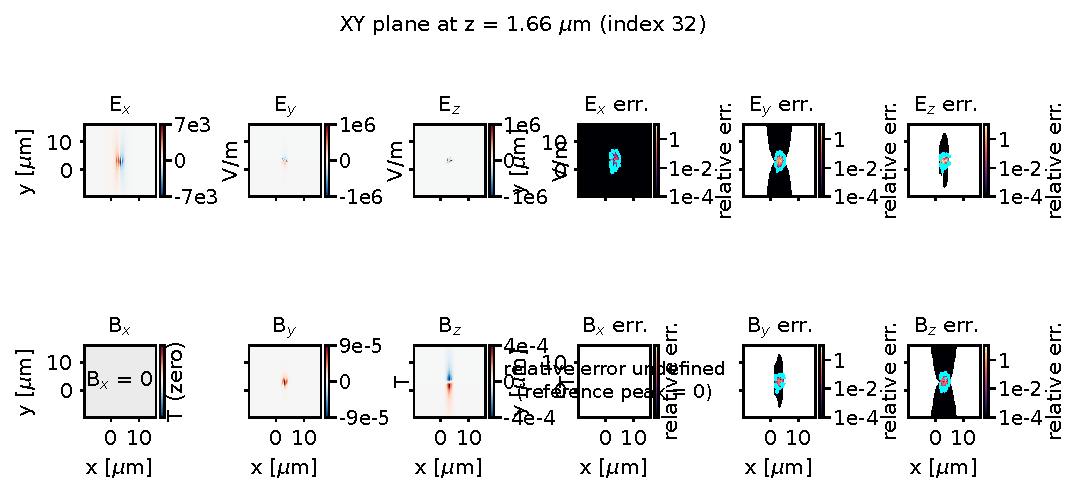
\includegraphics[width=\linewidth]{figs/large_sxy_g10.pdf}
\caption{Large-domain slices ($\gamma=10$, $128\times128\times64$, cell
$2\times10^{-7}$\,m, $N=100$, JURECA H100), axial-$x$ geometry: the bunch
moves along $+x$, so $B_x$, the component along the propagation axis, is
identically zero. In the x-y cut the beam axis $x$ is horizontal; the z-y
cut is a transverse view with the beam axis $x$ perpendicular to the page,
so the horizontal axis is the transverse $y$, not the propagation direction,
and $z$ is vertical. The x-y plane is shown; the z-y plane is continued in
Fig.~\ref{fig:large}. \densityrow{} Below the density row, each image
carries the electric block first and the magnetic block second.
The electric block shows four columns $E_x,E_y,E_z,E^2$: the three
components share one symmetric-logarithmic scale and bar (peak in percent of
the shared maximum), $E^2$ has its own logarithmic scale and unit label, and
a logarithmic error row against the order-4 driver reference lies beneath.
$E_x$ is suppressed but nonzero, peaking at $0.5475\%$ (x-y) and $0.1384\%$
(z-y) of the shared maximum. The magnetic block shows the same
four-column layout and error convention for $B_x,B_y,B_z,B^2$. For uniform
motion along $+x$ the field is purely transverse, so $B_x$ is identically
zero: its field panel is blank and its error panel is fully masked, since
the relative error of an identically zero component is undefined. The
magnetic plane peak is $1.5\times10^{-4}$\,T (x-y) and $1.4\times10^{-4}$\,T
(z-y). Grey pixels are masked.}
\label{fig:large}
\end{figure}

\begin{figure}[t]
\ContinuedFloat
\centering
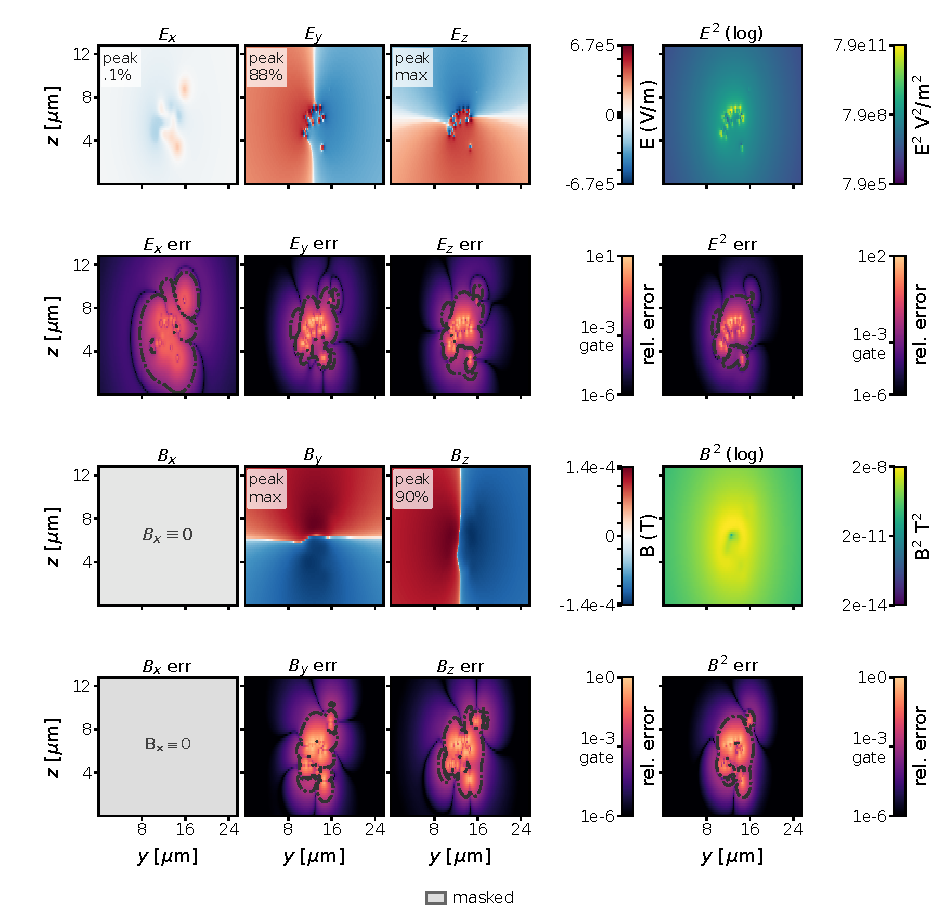
\includegraphics[width=\linewidth]{figs/large_szy_g10.pdf}
\caption{Large-domain slices (continued): z-y plane at
$\gamma=10$, with the same electric/magnetic blocks, colour scales, masks
and error conventions as the x-y plane in Fig.~\ref{fig:large}.}
\end{figure}

\begin{figure}[t]
\centering
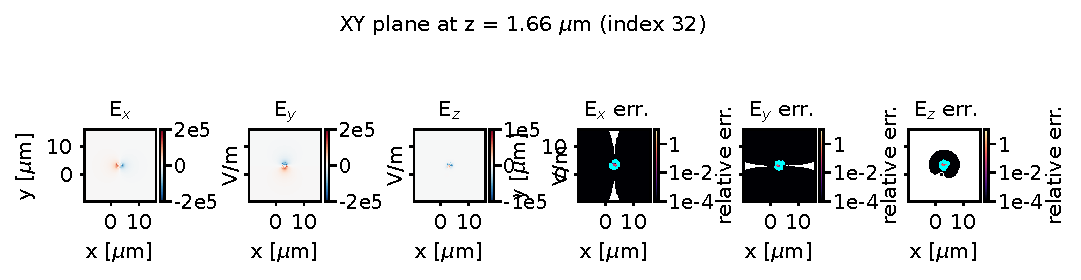
\includegraphics[width=\linewidth]{figs/large_sxy_g1.pdf}
\caption{Large-domain slices for the stationary bunch ($\gamma=1$), same
domain and layout as Fig.~\ref{fig:large}. In the x-y cut $x$ is horizontal;
the z-y cut is the same transverse view as in Fig.~\ref{fig:large}, with $x$
perpendicular to the page, $y$ horizontal and $z$ vertical; the bunch is
stationary, so it has no propagation direction. \densityrow{} The x-y plane
is shown; the z-y plane is continued in Fig.~\ref{fig:largeg1}. Below the
density row, each image has the electric block first
and the magnetic field row second. The electric block shows four columns $E_x,E_y,E_z,E^2$: the three
components share one symmetric-logarithmic bar (peak in percent of the
shared maximum), $E^2$ has its own logarithmic scale and unit label, and a
logarithmic error row lies beneath. The core error reaches
$8.4\times10^{-1}$ (z-y $E_x$), far above the $10^{-3}$ gate. The magnetic
field row shows four columns $B_x,B_y,B_z,B^2$; the stationary reference
magnetic field is identically zero, so every magnetic field panel is blank.
The magnetic error row is omitted because the relative error of an
identically zero component is undefined, as in the per-$\gamma$ $\gamma=1$
figure. Grey pixels are masked.}
\label{fig:largeg1}
\end{figure}

\begin{figure}[t]
\ContinuedFloat
\centering
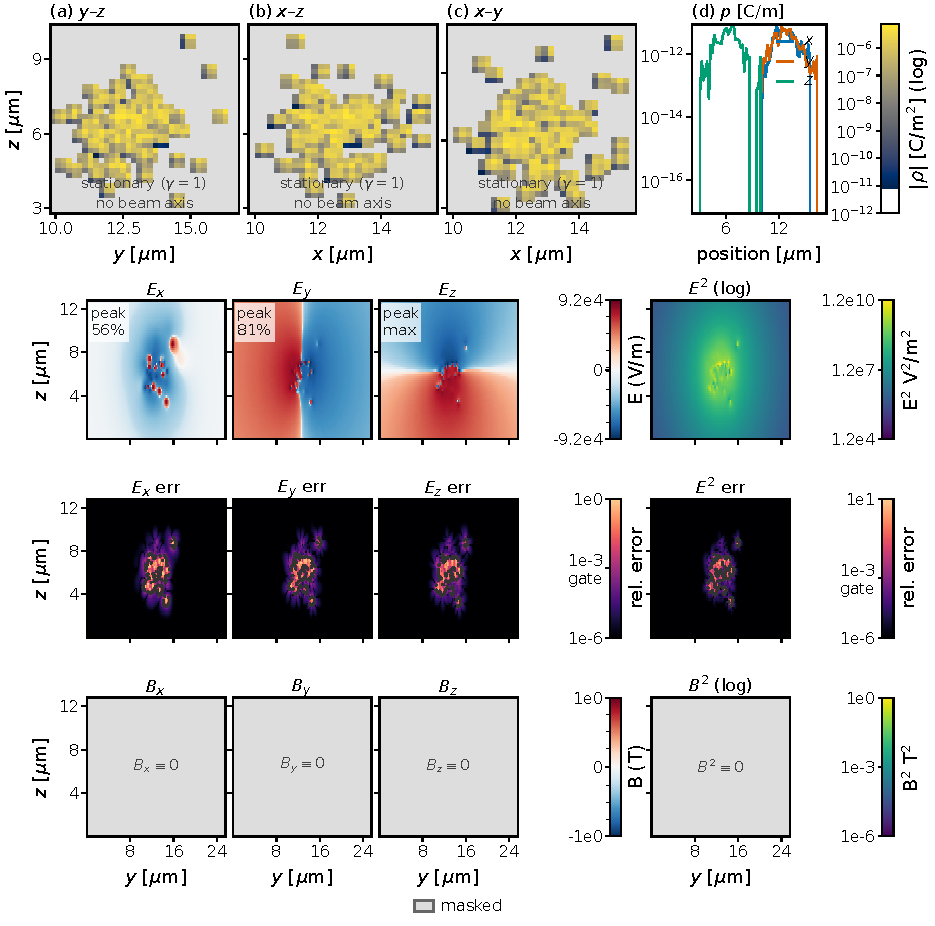
\includegraphics[width=\linewidth]{figs/large_szy_g1.pdf}
\caption{Large-domain slices for the stationary bunch (continued): z-y
plane, with the same blocks, colour scales, masks and error conventions as
the x-y plane in Fig.~\ref{fig:largeg1}.}
\end{figure}
